Después de analizar detenidamente los requisitos se procede a detallar la solución propuesta para el desarrollo de Vihrtual-App.

\subsection{Conjunto de entrenamiento}
El grueso del desarrollo se va a centrar en trabajar con el conjunto de preguntas y respuestas facilitado por parte de la Unidad de Enfermedades Infecciosas del Hospital General de Elche para generar un primer conjunto de entrenamiento o \textit{dataset}. Se propone empezar por un subconjunto de ellas e ir ampliándolo a lo largo del desarrollo. El principal trabajo en esta fase se centra en generar distintas variaciones (30 aprox.) de las preguntas para asegurar un amplio espectro de reconocimiento.\\

Por otra parte se observa que las respuestas proporcionadas son en muchos casos de difícil asimilación por parte de los usuarios. Por tanto, es necesario dinamizar estas respuestas para no aburrir al usuario e intentar captar su intención. Esta tarea se realizará mediante la introducción modificaciones tales como:

\begin{itemize}
	\item División de las respuestas más largas en varios mensajes.
	\item Ligeros cambios para variar el registro a otro menos formal.
	\item Eliminar afirmaciones y negaciones rotundas para adaptar las respuestas a una mayor variedad de preguntas.
	\item Hacer uso de algunos emoticonos para acompañar a ciertas expresiones o datos.
\end{itemize}

\subsection{Interacción}
[TODO: características sociales del bot, personalidad, elementos visuales, respuestas rápidas, avatar ...]


\subsection{Aspectos técnicos}
Tras el análisis realizado en la sección \ref{herramientas construir chatbots} sobre diferentes \textit{frameworks} para construir chatbots se escoge a \textit{Rasa} como plataforma sobre la cual se realizará el desarrollo. Las razones detrás de esta elección son las siguientes:\\ 

\begin{itemize}
	\item \textit{Rasa} cuenta con todas las herramientas necesarias para la correcta interpretación de las intenciones del usuario mediante técnicas de \textit{NLU} y noción del contexto.
	\item Es \textit{opensource}, gratuito y a diferencia de sus competidores, no se basa en ningún servicio en la nube propietario. Esto permite realizar el despliegue completo de la plataforma en cualquier máquina. 
	\item  En consecuencia, se obtiene independencia de otros servicios y control total sobre los datos recopilados de conversaciones, pues estas no estarán en manos de terceros.
	\item La plataforma ofrece una herramienta adicional para el aprendizaje supervisado llamada \textit{Rasa X}. Esta permite realizar fácilmente la revisión y etiquetado de las conversaciones por lo que resulta idónea para el desarrollo.
\end{itemize}	

\subsection{Distribución}
Teniendo en cuenta el carácter del servicio se propone que el chatbot se ponga a disposición del público a través de una web de libre acceso y sin requerir registro. El objetivo es facilitar a los usuarios el acceso  y esta opción hará que cualquier persona pueda acceder al servicio sin necesidad de introducir ningún dato personal ni instalar ninguna aplicación en su terminal. \\

Para aquellos usuarios que lo deseen se empaquetará la web en una aplicación tanto para \textit{Android} como para \textit{iOS} utilizando el framework \textit{Capacitor}. Esto permite que aquellos usuarios interesados puedan instalar el servicio desde las tiendas de aplicaciones habituales en sus dispositivos móviles.\\

\subsection{Roadmap}
Siguiendo la metodología \textit{Scrum} se propone una ruta de desarrollo (ver figura \ref{fig:roadmap desarrollo}) centrada en la obtención de un producto mínimo viable lo antes posible. Para ello primeramente se realizan los diseños del chatbot, se organiza la información recibida y se trabaja para la obtención de un \textit{PMI} en versión web. A partir de ese punto es se publica una versión de prueba del \textit{bot} para empezar con la obtención de datos reales  y realizar distintas iteraciones sobre el producto hasta conseguir el resultado deseado. Una vez se alcanza el nivel de madurez requerido, la web se empaqueta como \textit{app} para móvil y se publica.\\

\begin{figure}[htbp]
\centering
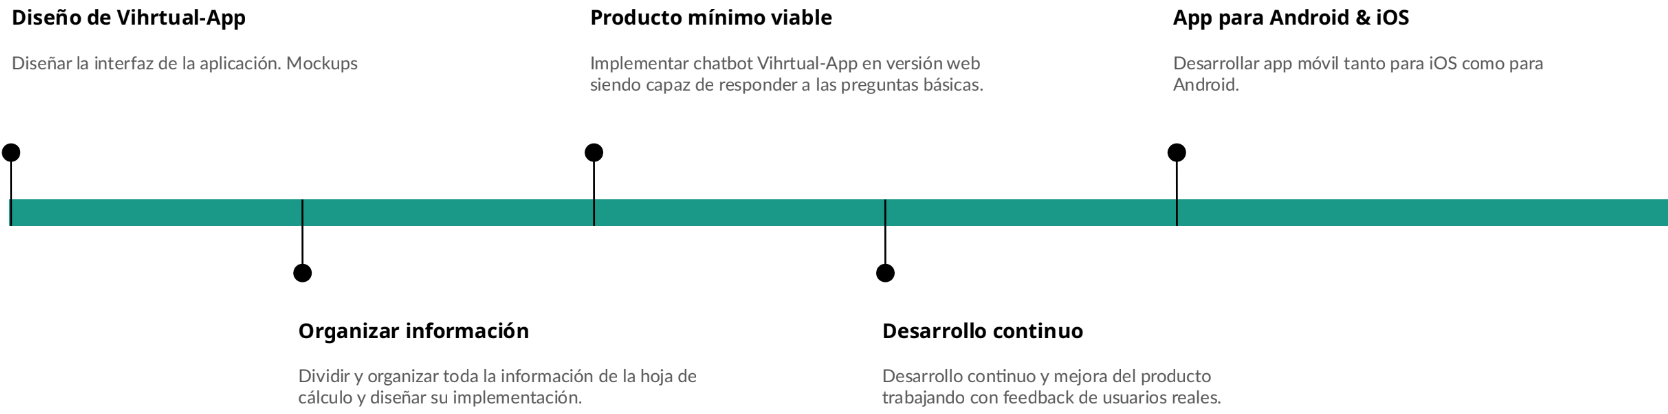
\includegraphics[scale=0.4]{../images/roadmap.png} 
\caption{\textit{Roadmap} propuesto para el desarrollo de Vihrtual-App}
\label{fig:roadmap desarrollo}
\end{figure}

Este propuesta se presenta en una reunión con los colaboradores la Unidad de Enfermedades Infecciosas del Hospital General de Elche para obtener su aprobación. Tanto las notas de la reunión como las diapositivas se pueden encontrar en los documentos anexos a este trabajo.\\